\section{Topology and Geometry}

% \subsection{Mesh topology}
While mesh geometry describes the location of mesh vertices in space, mesh topology indicates 
how vertices are connected to each other by edges, triangles or any type of mesh element. 
Both information are required on a computational mesh to perform mesh visualization,
mechanical modeling, collision detection, haptic rendering, scalar
or vectorial field description.

%Since topological changes are essential for surgery simulators, a common difficulty when designing those simulators is to ensure that the visual, mechanical, haptic and collision behavior of all meshes stay valid and consistent upon any topological change. 

% We handle topological changes in a modular and versatile way. Modular since each SOFA component (collision detection, mechanical solver$\ldots$) may be written with little knowledge about the nature of other components; versatile because any type of topological changes can be handled with the proposed design. 

Keeping a modular design implies that mesh related information (such as mechanical or visual properties) is not centralized in a single  mesh data structure but is instead spread out in the software components that are using this information.
% \\
% \textbf{\textit{Family of topologies}}\\
We consider meshes that are cellular complexes made of $k$-simplices (triangulations, tetrahedralisation) or $k$-cubes (quad or hexahedron meshes). These meshes are the most commonly used in real-time surgery simulation and can be hierarchically decomposed into $k$-cells, edges being $1$-cells, triangles and quads being $2$-cells, tetrahedron and hexahedron being $3$-cells. 
To take advantage of this feature, the  different mesh topologies are structured as a family tree (see Fig.~\ref{fig:BW_Topology_Family_Tree}) where children topologies are made of their parent topology. This hierarchy makes the design of simulation components very versatile since a component working on a given mesh topology type will also work on its derived types. For instance a spring-mass mechanical component only requires the knowledge of a list of edges (an \textit{EdgeSetTopology} as described in Fig.~\ref{fig:BW_Topology_Family_Tree}) to be effective. With this design, a spring-mass  component can be used at no additional cost on triangulation or hexahedral meshes that derive from an \textit{EdgeSetTopology} mesh.
 
%The proposed hierarchy makes also a distinction between conformal and manifold meshes. While most common FEM components require a mesh to be conformal (but not necessarily manifold), many high-level software components (such as cutting, contact, haptic feedback algorithms) require the mesh to be a manifold where a surface normal is well-defined at each vertex.   
\begin{figure}[ht]
    \centering
        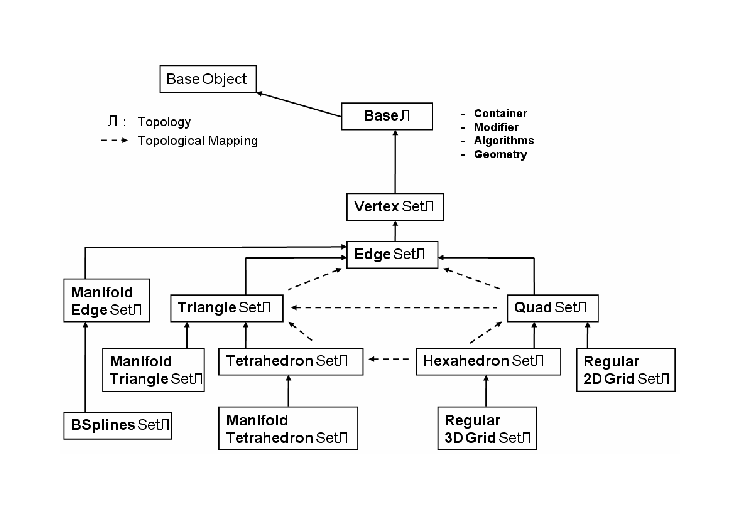
\includegraphics[width=0.9\textwidth]{BW_Topology_Family_Tree}
       \caption{Hierarchy of mesh topology. Dashed arrows indicate possible  \textit{Topological Mappings} from a topology object to another.}
    \label{fig:BW_Topology_Family_Tree}
\end{figure}


Topology objects are composed of four functional members:
 \textit{Container},  \textit{Modifier},  \textit{Algorithms} and  \textit{Geometry}.
The  \textit{Container} member creates and updates when needed two complementary arrays. The former describes the $l$-cells included in a single $k$-cell, $l<k$, while the latter gives the $k$-cells adjacent to a single $l$-cell.
From these arrays, generic methods give access to both full topological element description and complete adjacency information.
The  \textit{Modifier} member provides low-level methods that implement
elementary topological changes such as the removal or addition of an element. The  \textit{Algorithms} member provides high-level topological modification methods (cutting, refinement) which
decompose complex tasks into low-level
ones). 
The  \textit{Geometry} member provides geometrical information about the mesh (e.g. length, normal, curvature, ...) and requires the knowledge of the vertex positions stored in the  \textit{Degrees of Freedom} component. \\
%Note that these high-level changes may need geometrical information, such as mesh refining, triangular surface cutting or tetrahedra removal in a given region of interest.

\begin{figure}[ht]
    \centering
        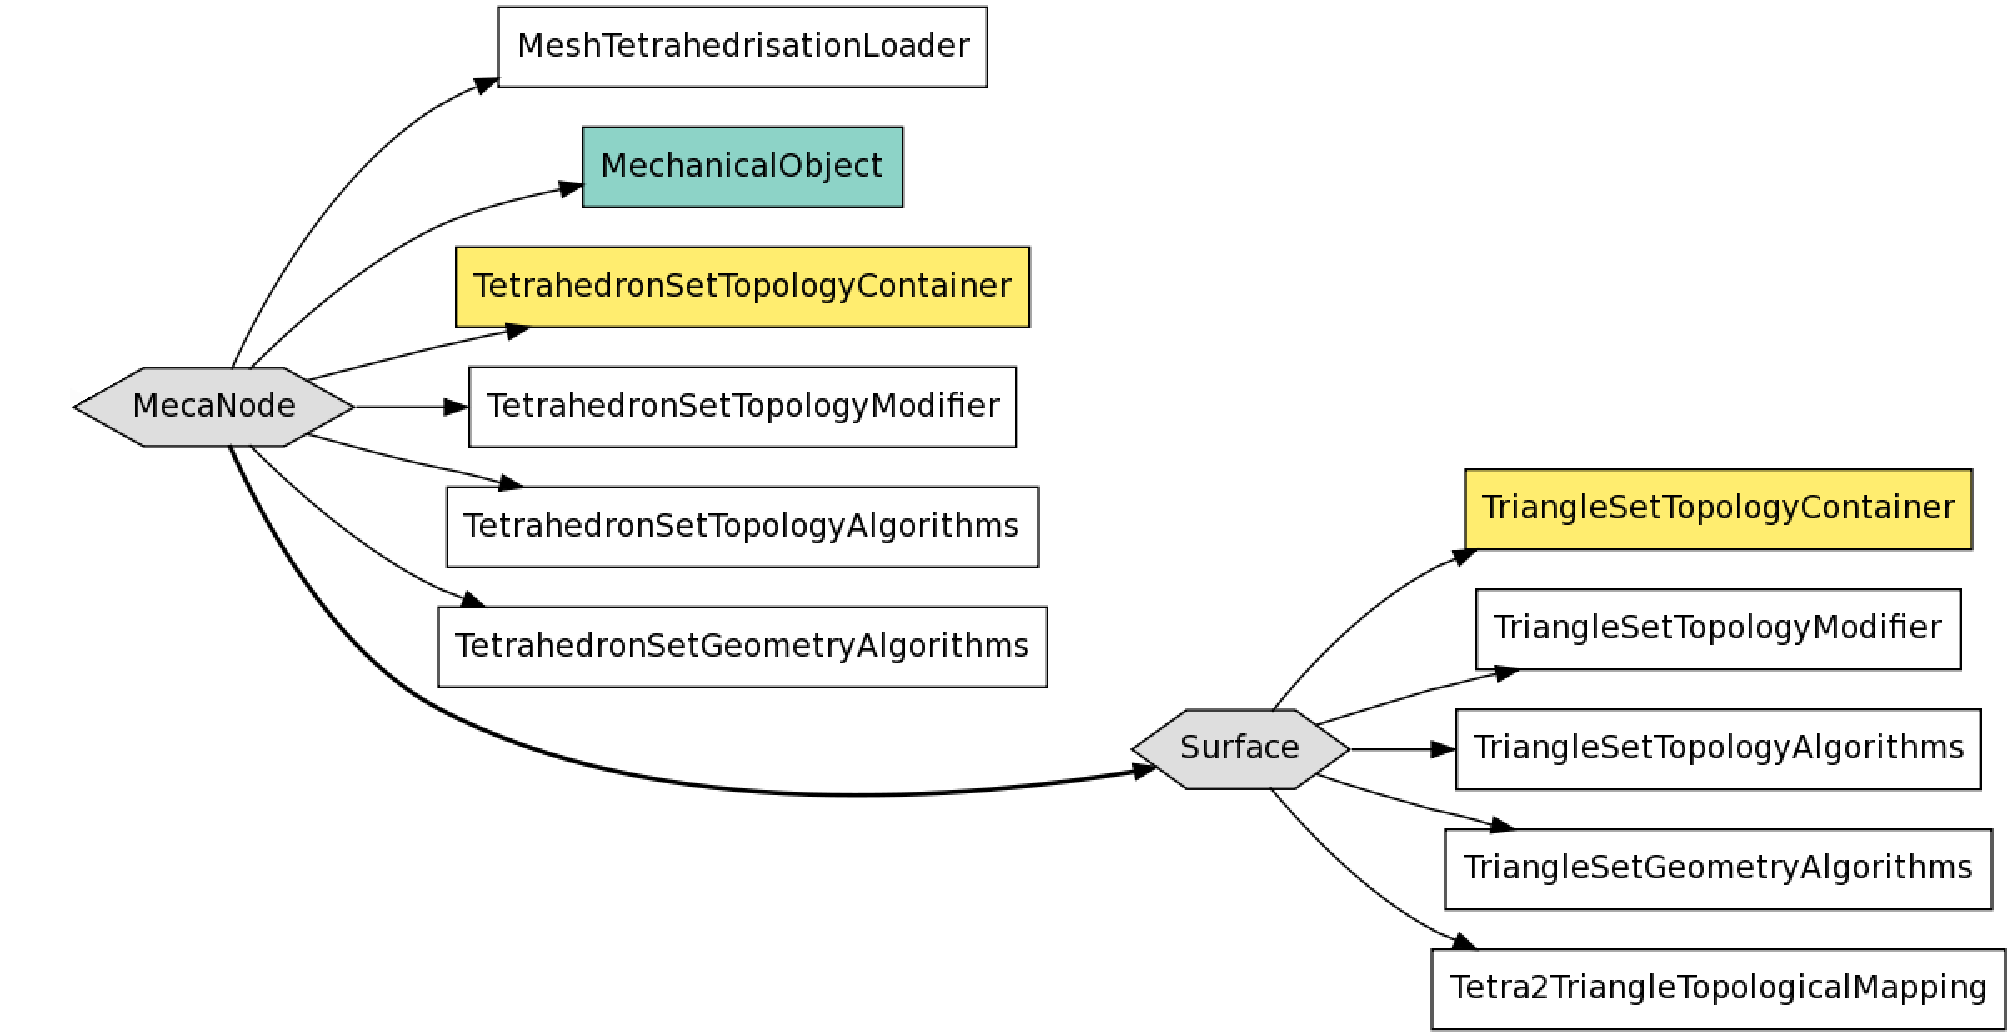
\includegraphics[width=0.9\textwidth]{topologyGraph.pdf}
       \caption{Scene Graph of a simple tetrahedral mesh where a topological mapping is defined to have the set of triangles located at the surface of the volumetric mesh.}
    \label{graphExample}
\end{figure}


Another important concept introduced in SOFA is the notion of \textit{Topological Mapping}. Those mappings  define a mesh topology in a from another mesh topology using the same DOFs.  For instance, one may need to apply specific forces on the surface bounding a volume (for instance to model the Glisson capsule surrounding the liver parenchyma). In this context, a \textit{Tetra2TriangleTopologicalMapping} may be used  to generate in a subnode the list of triangles on the border of a tetrahedral surfaces (see Figure \ref{graphExample}). Similarly, one may obtain the set of edges bordering a triangular mesh or the set of quads at the surface of an hexahedral mesh. Topological mapping may be used to split topological cells into other types of cells. Thus, a quad may be split into 2 triangles and an hexahedron into 5 or 6 tetrahedra. Specific mapping components exist to create an tetrahedral mesh from a set of hexahedra or to create triangular meshes from quads.

%An example of graph with Tetrahedral and Triangular Topology objects is given Fig. \ref{graphExample}. It also contains a mapping from the tetrahedral topology to the triangular one. 


\begin{figure}[ht]
    \centering
        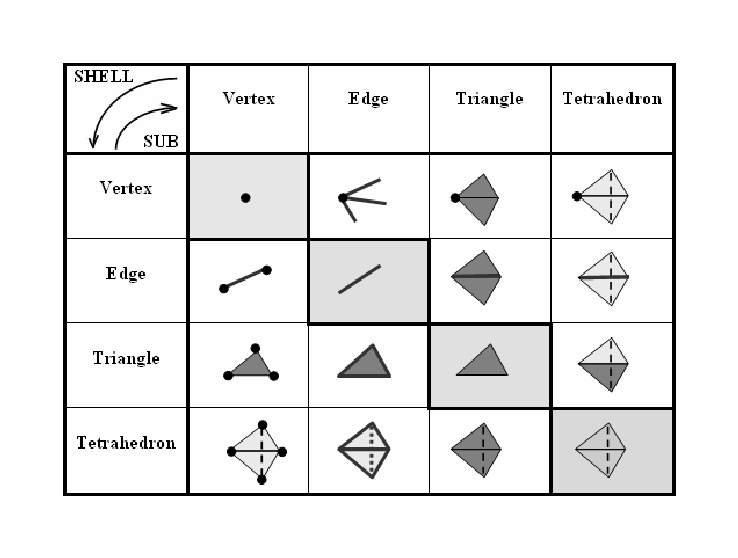
\includegraphics[width=0.8\textwidth]{BW_Sub_Shell_Diagram}
  %  \caption{Diagram of topological information for the elements of type Vertex, Edge, Triangle and Tetrahedron. \textit{ Sub Elements} (\textit{ bottom-left}) and \textit{ Shell Elements} (\textit{ top-right}) are stored in the \textit{ Container}. At each index $i$: \textit{ AB-Sub} array stores the indices vector of the elements of type \textit{ B} that compose the element of type \textit{ A} indexed by $i$; \textit{ AB-Shell} array stores the indices vector of the elements of type \textit{ A} that are adjacent to the element of type \textit{ B} indexed by $i$.}
    \caption{The two topological arrays stored in a \textit{ Container} correspond to the upper and lower triangular entries of this table. The upper entries provide the $k$-cells adjacent to a $l$-cell, $l<k$. The lower entries describe the $l$-cells included in a $k$-cell. Similar table exists for quad and hexahedron elements.}
    \label{fig:BW_Sub_Shell_Diagram}
\end{figure}

\subsubsection*{Mesh Data Structure}


% Choices of implementation
Containers storing mesh information (material stiffness, list of fixed vertices, nodal masses, ...) are stored in \textit{ components} and are spread out in the simulation tree.  
Most containers are simple arrays  with contiguous memory storage and a short direct access time.
This is important for real-time simulation, but bears some drawbacks when elements of these arrays are being removed since it entails the renumbering of elements. 
%For instance, when a single element is removed, the last array element is renumbered such that the array stays contiguous. 
Fortunately, all renumbering tasks that maintain consistent arrays can be automated and hidden to the user when topological changes in the mesh arise. 
Therefore, efficient access of  mesh data structures is granted while the complexity of keeping the container consistent with topological changes is automated.

There are as many containers as topological elements, currently: vertices, edges, triangles, quads, tetras, hexas. These containers are similar to the STL \textit{ std::vector} classes and allow one to store any component-related data structure. A typical implementation of spring-mass models would use an edge container that stores for each edge, the spring stiffness and damping value, the $i^{th}$ element of that container being implicitly associated with the $i^{th}$ edge of the topology. Finally, two other types of containers with similar characteristics have been defined. The former stores a data structure for a subset of topological elements (for instance pressure on surface triangles in a tetrahedralisation) while the latter stores only a subset of element indices.\\


%\subsubsection{Handling Topological Changes}\label{sec:topologicalChanges}

% to reformulate

% So as to make this design compatible with topological changes at each time step of the simulator,
% consistency has to be maintained for all components that rely on topology information, by applying the observer design pattern to the data structure.

% \subsection{Concept of Topological Event}

% \noindent % Order to respect when adding or removing an element (low-level methods)
% Motivation : topological changes are handled in a transparent way for the user through a mechanism of propagation of topological events from the topological components %toward other components.
%Surgery simulation involves complex topological changes on meshes, 
%for example when cutting a surface along a line segment, or when locally refining a volume before removing some tissue.
%However, one can always decompose these complex changes into a sequence of elementary operations, 
%such as adding an element, removing an element, renumbering a list of elements or modifying a vertex position.
%
%The approach used in \sofa to handle topological changes makes the  update of data structures transparent to the user, through a mechanism of propagation of topological events.
%A topological event corresponds to the intent to add or to
%remove a list of topological elements. But the removal of elements cannot be tackled in the same way as the addition of elements. Indeed, the element removal event must be first notified to
%the other components before the element is actually removed by the \textit{Modifier}.
%Conversely, element addition is first processed by the \textit{Modifier} and then element addition event is notified to other components.
%Besides, the events notifying the creation of elements also include a list of ancestor elements. Therefore, when splitting one triangle into two sub-triangles, each component-related information (\textit{ e.g.} its Young modulus or its mass density) associated with a sub-triangle will be created knowing that the sub-triangle originates from a specific triangle. Such mechanism is important to deal with meshes with non-homogeneous characteristics related to the presence of pathologies.
%
%\vspace{-0.5cm}
%
%\begin{figure}[ht]
%    \centering
%      %  \mbox{
%      %  \includegraphics[width=0.5\textwidth]{Handling_Topological_Changes}
%      %    \includegraphics[width=0.5\textwidth]{Triangle_Splitting}
%      %  }
%        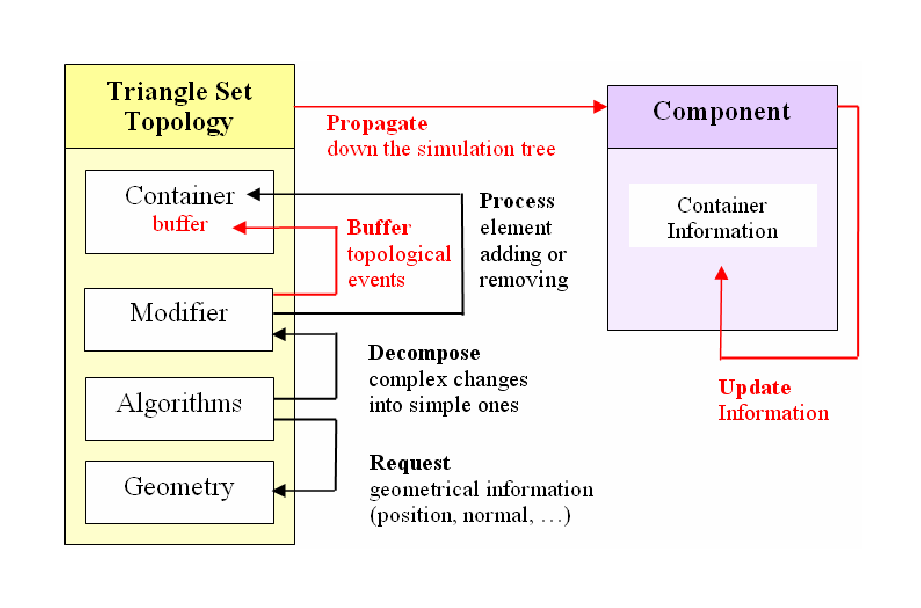
\includegraphics[width=0.8\textwidth]{Handling_Changes}
%    \caption{Handling topological changes, with the example of a \textit{Triangle Set Topology}. 
%   \textit{Component} corresponds to any component of the simulation which may need topological information to perform a specific task.
%    Black features indicate the effective change process. Red features show the steps of event notification.}
%    \label{fig:Handling_Changes}
%\end{figure}


% \vspace{-1.5cm}

%\begin{figure}[ht]
%    \centering
      %  \mbox{
      %  \includegraphics[width=0.5\textwidth]{Handling_Topological_Changes}
      %    \includegraphics[width=0.5\textwidth]{Triangle_Splitting}
      %  }
%        \includegraphics[width=0.65\textwidth]{Triangle_Splitting}
%    \caption{Seven steps to split one triangle into two sub-triangles.}
%    \label{fig:Triangle_Splitting}
%\end{figure}

%The mechanism to handle topological changes is illustrated by Fig.~\ref{fig:Handling_Changes}.
%The notification step consists in accumulating the sequence of
%topological events  involved in a high-level topological change into a buffer stored in
%the \textit{ Container}. Then the event list is propagated to all its
%neighbors and leaves beneath by using a visitor mechanism, called a
%\textit{ Topology Visitor}. Once a given component is visited, the topological
%events are actually processed one by one and the data structure used to store mesh related information are automatically updated.
%
%In practice, for each specific component (\textit{ e.g.} spring-mass mechanical component), a set of callback functions are provided describing how to update the data structure (\textit{ e.g.} spring stiffness and damping values) when adding or removing an element (\textit{ e.g.} the edges defined by the two extremities of the springs).
%We applied the observer design pattern so that component-related data structures update themselves automatically.


